\documentclass[11pt, thmnum, eqsecnum, allcites, dark]{mathbeamer}
%%%%%%%%%%%%%
%% Options %%
%%%%%%%%%%%%%
%% thmnum: numbered theorems
%% eqsecumn: number equaiton with section
%% authoryear: author-year style reference
%% allcites: output all the reference in bib.bib
%% dark: use dark color style
%% light: use light color style
%% nds: not use the default setting

%%%%%%%%%%%%%%%%%%%%%%%%%%%%%%%%%%%%%%%%%%
%===========================
% your definitions:
%===========================
%===================================
%% Self defined command
%===================final options====================

% ------------------设置用acrobat打开就会全屏显示  
%\hypersetup{pdfpagemode=FullScreen}

%--------------------是否逐条显示--------------------
%\beamerdefaultoverlayspecification{<+->}



%================packages===============================
%%已有的package:
%hyperref, mathtools, bm
%babel
%amsrefs
\usepackage{float}
\usepackage{multirow}%表格
\usepackage{latexsym}
\usepackage{amsmath,amssymb}
\usepackage{color,xcolor}
\usepackage{algorithm}
\usepackage{amsthm}
\usepackage{graphicx}%图表
\usepackage{wrapfig}%图表
\usepackage{supertabular}
\usepackage{harvard}%citation宏包
\usepackage{xeCJK}


%======================================================
%-----------------------others---------------------------
\newcommand{\eps}{\varepsilon}%简化$\varepsilon$的表示
%================theorem environments==========
%% Note: the following theorem environments
%%       already defined in mathbeamer.cfg
%%       Not need to define it again
%%\theoremstyle{plain}
%%\newtheorem{thm}{Theorem}[section]
%%\newtheorem{lem}[thm]{Lemma}
%%\newtheorem{prop}[thm]{Proposition}
%%\newtheorem{cor}[thm]{Corollary}
%%\theoremstyle{definition}
%%\newtheorem{defn}[thm]{Definition}
%%\theoremstyle{example}
%%\newtheorem{conj}{Conjecture}
%%\newtheorem{exmp}{Example}
%%\newtheorem*{rmk}{Remark}
%%\theoremstyle{break}
%%\newtheorem{bthm}{Theorem}[section]
%%\newtheorem{blem}[thm]{Lemma}
%%\newtheorem{bprop}[thm]{Proposition}
%%\newtheorem{bcor}[thm]{Corollary}
\newcommand{\mthm}{Theorem}
%===================================================
%---------------------------中文字体
\setCJKmainfont[BoldFont={NotoSerifCJKsc-Bold}]{NotoSerifCJKsc-Regular}
\setCJKsansfont{NotoSerifCJKsc-Regular}

%----------------------行距
%\linespread{1.3}

%=========================preferences==========================
%---------------item的符号改为三角形
\setbeamertemplate{items}[triangle]%[circle,ball,]

%----------------citation
\citationstyle{dcu}%-----author,year
%\bibliographystyle{}

%======================at documents===================================

\AtEndDocument{%
	%========================
	% thanks
	%========================
	\section{Thanks}
	\newcounter{ffn}
	\setcounter{ffn}{\value{framenumber}}
	\renewcommand{\insertframenumber}{\inserttotalframenumber}
	\begin{frame}
	\begin{center}
		\LARGE{\bfseries
			Thanks!
		}
	\end{center}
\end{frame}
%========================
% bibliography
%========================
\section{Reference}
\begin{frame}[t, allowframebreaks]{Reference}
\bibliography{slides/bib}
\end{frame}
\setcounter{framenumber}{\value{ffn}}
}





%===========================
% your title/name/institute:
%===========================
\title[\sc Mean Curvature Flow \& Ricci Flow]{\sc On the Evolution of Mean Curvature Flow\\ with Background Ricci Flow}
\author{Stu Name}
\date{\today}
\institute[USTC]{School of Mathematical Sciences, USTC}

\begin{document}
%===========================
% your slides:
%===========================
%--------------------生成目录页,目录太长时加选项[shrink]
	\begin{frame}{\sc{Contents}}
	\addtocounter{framenumber}{-2}%-----------位置放在beginframe之后,不然无效
	\thispagestyle{empty}
	\tableofcontents[hideallsubsections]    
	% 也可以插入选项 [pausesections]
	%列目录时,隐藏所有的小节\tableofcontents[hideallsubsections]
	\end{frame}


%===========================
% example slides:
%===========================
%\section{Overview}
\label{section1}
\begin{frame}{Overview}
\begin{itemize}[<+->]
 \item The trivial Set Cover algorithm has running time of ${\cal O}(2^n)$.
 \item bla, bla, bla\ldots
\end{itemize}

\end{frame}


%\section{Blocks}
% --------------------------------------------------- Slide --
\subsection{Blocks}
\label{blocks}
\begin{frame}{Blocks}
  \begin{block}{Block Title}
    Lorem ipsum dolor sit amet, consectetur adipisicing elit, sed do eiusmod tempor incididunt ut labore et dolore magna aliqua.
  \end{block}
  \begin{alertblock}{Alert Block Title}
    Lorem ipsum dolor sit amet, consectetur adipisicing elit, sed do eiusmod tempor incididunt ut labore et dolore magna aliqua.
  \end{alertblock}
\end{frame}

%\section{Columns}
% --------------------------------------------------- Slide --
\subsection{Columns}
\label{columns}
\begin{frame}{Columns}
  \begin{columns}
    \column{0.5\textwidth}
      Lorem ipsum dolor sit amet, consectetur adipisicing elit, sed do eiusmod tempor incididunt ut labore et dolore magna aliqua.
    \column{0.5\textwidth}
      Lorem ipsum dolor sit amet, consectetur adipisicing elit, sed do eiusmod tempor incididunt ut labore et dolore magna aliqua.
  \end{columns}
\end{frame}

%\section{Description}
% --------------------------------------------------- Slide --
\subsection{Description}
\label{description}
\begin{frame}{Description Environment}
  \begin{description}
    \item[API] Application Programming Interface
    \item[LAN] Local Area Network
    \item[ASCII] American Standard Code for Information Interchange
  \end{description}
\end{frame}

%% -*- coding: utf-8 -*-
\section{Definition}
% --------------------------------------------------- Slide --
\subsection{Definition}
\label{definition}
\begin{frame}{Definition}
  Then there’s the definition environment which produces a standard color block but with the title already specified as ‘definition’.
  \begin{semiverbatim}
    \\begin\{definition\}\newline
    A prime number is a number that...\newline
    \\end\{definition\}
  \end{semiverbatim}
  \begin{definition}
    A prime number is a number that...
  \end{definition}
\end{frame}
\subsection{Custom definition}
\begin{frame}{Custom definition}
  You can also use the custom definition defined in ``slides/usrdef.tex'', for example
  \begin{semiverbatim}
    \\begin\{defn\}\newline
    A prime number is a number that...\newline
    \\end\{defn\}
  \end{semiverbatim}
  \begin{defn}
    A prime number is a number that...
  \end{defn}
\end{frame}

\section{MATH EQUATIONS}
\begin{frame}{NOTE}
\begin{itemize}
	\item $\ allowdisplaybreaks[n]$\\
	n的值为0到4,表示分页的坚决程度,例如0表示能不分页就不分页,4表示强制分页。\\
\end{itemize}

\end{frame}

\begin{frame}{items}
	usepackage[namelimits]{amsmath} 数学公式\\
	usepackage{amssymb}             数学公式\\
	usepackage{amsfonts}            数学字体\\
	usepackage{mathrsfs}            数学花体\\
	enumerate标序
	\begin{enumerate}
	\item 经营人员M作为委托人
	\item 生产成员P作为委托人
	\item 他们作为合伙人互相监督、分享风险
	\end{enumerate}
	itemize不标序
	\begin{itemize}
	\item good1
	\item good2
	\end{itemize}
\end{frame}	

\subsection{大公式环境}
\begin{frame}{各种公式环境}
	行内公式\\
	$ a+b=c $,$ 25\% $,$ \{a,b\} $\\

	\vspace{1em}
	行间公式,tag并label
	\[x+y=z \tag{1.1}\label{1.1}\]

	\text{\$ equation \$}\\
	\text{\$\$ equation \$\$}\\
	\text{/$[ equation /$]}\\
	他们都不产生编号公式。后两种公式单独占一行,即不能嵌入正文中。\\
	用\text{\$\$}表示的公式自动居中,而\text{/$[ /$ ]}表示的公式会根据配置的全局对齐方式对齐。
\end{frame}


\begin{frame}{标准单个公式环境}
	begin\{equation\}\\
	...\\
	end\{equation\}\\
	它是最一般的公式环境,表示一个公式,默认情况下之表示一个单行的公式,但是它的功能可以通过内嵌各种其他环境进行扩展。\\
	它可以内嵌的一些关于对齐的环境将在后面介绍。
\end{frame}
	
\begin{frame}[shrink]
	\begin{tabular}{lp{5cm}p{4cm}}
		\hline Environment name &Description &Notes\\
		\hline eqnarray and eqnarray*	&Similar to align and align*	&Not recommended since spacing is inconsistent\\
		\hline multline and multline*	&First line left aligned, last line right aligned	&Equation number aligned vertically with first line and not centered as with other environments.\\
		\hline gather and gather*	&Consecutive equations without alignment&\\	 
		\hline flalign and flalign*	&Similar to {\color{red}{align}}, but left aligns first equation column, and right aligns last column&\\ %空白列也必须加"&"
		\hline alignat and alignat*	&Takes an argument specifying number of columns. Allows to control explicitly the horizontal space between equations	&You can calculate the number of columns by counting \& characters in a line and adding 1\\
		\hline
	\end{tabular}
	表格引用自:\url{http://en.wikibooks.org/wiki/LaTeX/Advanced\_Mathematics}
	其中除了eqnarray是内置的以外,其他的都需要amsmath包支持。
	\end{frame}


\begin{frame}{align,多个公式}
	居中列两个公式,并且加*不自动编号\\
	与表格环境一样,它采用“\&”分割各个对齐单元,使用“$// $”换行。它的每行是一个公式,都会独立编号。
	\begin{align*}
		f(x) &= (x+a)(x+b) \\
			 &= x^2 + (a+b)x + ab\\
	\end{align*}
\end{frame}

\begin{frame}{eqnarray,多个公式}
	equation环境,自动编号(1)(2)(.)
	\begin{eqnarray}
	\alpha+\beta &=\gamma\\
	\varepsilon+\zeta+\eta &=\theta%这里加//会产生三行编号
	\end{eqnarray}
\end{frame}

\begin{frame}{gather,数学推导}
	它是最简单的多行公式环境,自己不提供任何对齐。其中的各行公式按照全局方式分别对齐。\\
	在设置了全局左对齐之后,因为不存在内部各个公式之间对排版的干扰,这种环境非常适合写数学推导或者证明。\\
	\begin{gather*}
	E(X)=\lambda	\qquad	D(X)=\lambda	\\
	E(\bar{X})=\lambda	\\
	D(\bar{X})=\frac{\lambda}{n}	\\
	E(S^2)=\frac{n-1}{n}\lambda	\\
	\end{gather*}
\end{frame}

\begin{frame}{alignat,多列公式对齐}
	它接收一个参数用来指定根据哪一列对齐。
	\begin{alignat}{2}
	 \sigma_1 &= x + y  &\quad \sigma_2 &= \frac{x}{y} \\  
	 \sigma_1' &= \frac{\partial x + y}{\partial x} & \sigma_2'
		&= \frac{\partial \frac{x}{y}}{\partial x}
	\end{alignat}

\end{frame}

\subsection{用于内嵌的对齐环境}
\begin{frame}
	这些环境无法独立构成一个数学环境,必须要嵌入在其他环境内部。
	\begin{tabular}{lp{7cm}}
		\hline Math environment name	&Description\\
		\hline gathered	&Allows to gather few equations to be set under each other and assigned a single equation number\\
		split	&Similar to align*, but used inside another displayed mathematics environment\\
		aligned	&Similar to align, to be used inside another mathematics environment.\\
		alignedat	&Similar to alignat, and just as it, takes an additional argument specifying number of columns of equations to set.\\
		
		\hline
	\end{tabular}

	\vspace{1em}
	表格引用自:\url{http://en.wikibooks.org/wiki/LaTeX/Advanced_Mathematics}.\\
	这些环境都需要amsmath包支持。
\end{frame}

\begin{frame}{内嵌split}
	它用于将一个公式拆分成多行,但是它整体还只是一个公式。\\可以用在equation,\$\$,\text{\ $[ \ $]}三个环境中,相当于align
	\begin{equation}
	 \begin{split}
	 (a + b)^4
	   &= (a + b)^2 (a + b)^2      \\
	   &= (a^2 + 2ab + b^2)	    	
		  (a^2 + 2ab + b^2)        \\
	   &= a^4 + 4a^3b + 6a^2b^2 + 4ab^3 + b^4\\
	 \end{split}
	\end{equation}
\end{frame}

\begin{frame}{内嵌aligned,多行对齐公式}
	\begin{equation}
		\left.\begin{aligned}
			   B'&=-\partial \times E,\\
			   E'&=\partial \times B - 4\pi j,
			  \end{aligned}
		\right\}
		\qquad \text{Maxwell's equations}
	   \end{equation}
	   left和right后加一个括号的表示用于自动调整各种括号的大小,必须配对使用。公式中的left. 是一个虚的left,目的是为了和right\}配对。
\end{frame}

\begin{frame}{内嵌array}
	用\&\&分开两列公式,rcl表示三列,分别右中左对齐
	\begin{equation}
		\omega_j=\left\{
		\begin{array}{rcl}
		\omega_j^s && b_i=0\\
		\omega_j^s+F_j(a_j^b) && b_i>0\tag{2.4}\label{2.4}	
		\end{array} \right.
		\end{equation}
\end{frame}
%% -*- coding: utf-8 -*-
\section{Example}
% --------------------------------------------------- Slide --
\subsection{Example}
\label{example}
\begin{frame}{Example}
  Next there’s the example environment which produces a block with the title ‘Example’.
  \begin{semiverbatim}
    \\begin\{example\}\newline
    Lorem ipsum dolor sit amet...\newline
    \\end\{example\}
  \end{semiverbatim}
  \begin{example}
    Lorem ipsum dolor sit amet, consectetur adipisicing elit, sed do eiusmod tempor incididunt ut labore et dolore magna aliqua.
  \end{example}
  As definition, you can also use the custom one ``examp'' which is defined in ``slides/usrdef.tex''.
\end{frame}

%\section{Figures}
% --------------------------------------------------- Slide --
\subsection{Figures}
\label{figures}
\begin{frame}\frametitle{Domination on a Chessboard}
  \begin{figure}[htb]
    \centering
    \begin{tabular}{cc}\pause{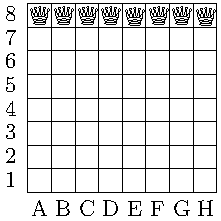
\includegraphics[scale=1]{examples/DomChess8.pdf}}&
      \pause{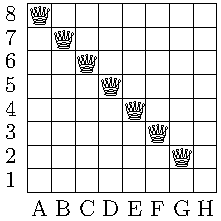
\includegraphics[scale=1]{examples/DomChess7.pdf}}\\
      \pause{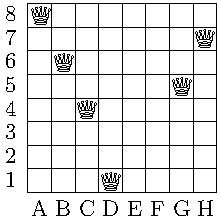
\includegraphics[scale=1]{examples/DomChess6.pdf}}&
      \pause{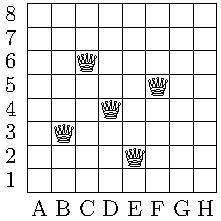
\includegraphics[scale=1]{examples/Chess1.pdf}}
    \end{tabular}
  \end{figure}
\end{frame}

% --------------------------------------------------- Slide --
%\subsection{Figures}
\label{figures2}
\begin{frame}\frametitle{Single figure with caption}
  \begin{figure}[htb]
    \centering
    
\includegraphics[scale=0.25]{examples/figures/400x400.png}
    \caption{This is an caption!}
  \end{figure}
\end{frame}

%\section{Hyperlinks}
% --------------------------------------------------- Slide --
\subsection{Hyperlinks Code}
\label{hyperlinks}
\begin{frame}{Hyperlink}
Before we can create any hyperlinks we need to tag the frames we want to link to using the \label command.

\hyperlink{contents}{click here}
\hyperlink{section1}{\beamerbutton{section 1 page}}
\hyperlink{columns}{\beamergotobutton{columns page}}
\hyperlink{figures}{\beamerskipbutton{pictures page}}
\hyperlink{figures}{\beamerreturnbutton{pictures page}}

\end{frame}

%\section{Lists}
% --------------------------------------------------- Slide --
\subsection{Itemize}
\label{itemize}
\begin{frame}{Lists - Itemize}
  \begin{itemize}
    \item Point A
    \item Point B
    \begin{itemize}
      \item part 1
      \item part 2
    \end{itemize}
    \item Point C
    \item Point D
  \end{itemize}
\end{frame}

% --------------------------------------------------- Slide --
\subsection{Pause}
\label{pause}
\begin{frame}{Lists - Itemize with Pause}
  \begin{itemize}[<+->]
     \item Point A
     \item Point B
    \begin{itemize}
       \item part 1
       \item part 2
    \end{itemize}
     \item Point C
     \item Point D
  \end{itemize}
\end{frame}

% --------------------------------------------------- Slide --
\subsection{Enumerate}
\label{enumerate}
\begin{frame}{Lists - Enumerate}
  \begin{enumerate}
    \item Point A
    \item Point B
    \begin{enumerate}
      \item part 1
      \item part 2
    \end{enumerate}
    \item Point C
    \item Point D
  \end{enumerate}
\end{frame}

% --------------------------------------------------- Slide --
\subsection{Enumerate (Roman Numerals)}
\label{enumerateRomanNumerals}
\begin{frame}{Lists - Enumerate (Roman Numerals)}
  \begin{enumerate} [(I)]
	\item Point A
	\item Point B
	\begin{enumerate} [(i)]
	  \item part 1
      \item part 2
	\end{enumerate}
	\item Point C
	\item Point D
  \end{enumerate}
\end{frame}

%\section{Tables}
% --------------------------------------------------- Slide --
\subsection{Tables}
\label{tables}
\begin{frame}{Tables}
  \begin{table}
    \begin{tabular}{l | c | c | c | c }
      Competitor Name & Swim & Cycle & Run & Total \\
      \hline \hline
      John T & 13:04 & 24:15 & 18:34 & 55:53 \\
      Norman P & 8:00 & 22:45 & 23:02 & 53:47\\
      Alex K & 14:00 & 28:00 & n/a & n/a\\
      Sarah H & 9:22 & 21:10 & 24:03 & 54:35
    \end{tabular}
    \caption{Triathlon results}
  \end{table}
\end{frame}

%% -*- coding: utf-8 -*-
\section{Theorem}
% --------------------------------------------------- Slide --
\subsection{Theorem Code}
\label{theoremCode}
\begin{frame}{Theorem}
  There is also a group of blocks that are especially useful for presenting mathematics. For example the ‘theorem’ environment, the ‘corollary’ environment and the ‘proof’ environment.
  \begin{semiverbatim}
    \\begin\{theorem\}[Pythagoras] \newline
      $ a^2 + b^2 = c^2$ \newline
    \\end\{theorem\} \newline
    \\begin\{corollary\} \newline
      $ x + y = y + x  $ \newline
    \\end\{corollary\} \newline
    \\begin\{proof\} \newline
      $\omega +\phi = \epsilon $ \newline
    \\end\{proof\}
  \end{semiverbatim}
\end{frame}

% --------------------------------------------------- Slide --
\subsection{Theorem Blocks}
\label{theoremBlocks}
\begin{frame}{Theorem Blocks}
  \begin{theorem}[Pythagoras]
    $ a^2 + b^2 = c^2$
  \end{theorem}
  \begin{corollary}
    $ x + y = y + x  $
  \end{corollary}
  \begin{proof}
    $\omega +\phi = \epsilon $
  \end{proof}
  As definition, you can also use the custom one ``thm/cor'' which is defined in ``slides/usrdef.tex''.
\end{frame}



%===========================
% bibliography
%===========================
%---\bibliography{slides/bib}%并没有cite但是参考文献全列出来了
%---usrdef.tex已经设定好了thanks和ref部分
\end{document}
